\documentclass[xcolor=dvipsnames]{beamer}
\usepackage[T1]{fontenc}
\usepackage[utf8]{inputenc}
\usepackage[english,slovak]{babel}

\usepackage{amsmath}
\usepackage{amsthm}
\usetheme{Pittsburgh}
\useoutertheme{shadow}

\usepackage{graphicx}
\usepackage{caption}
\usepackage{subcaption}

\usepackage[]{algorithm2e}
\usepackage{listings}
 \setbeamercovered{transparent}
 \usepackage{cuted}
\usepackage[export]{adjustbox}
\usepackage{mathtools}

\usepackage{lipsum}

\newcommand\Wider[2][3em]{%
\makebox[\linewidth][c]{%
  \begin{minipage}{\dimexpr\textwidth+#1\relax}
  \raggedright#2
  \end{minipage}%
  }%
}

%-------------------------------------------------------------------------------------
\title{\bf Convolutional neural network}
\author{Michal CHOVANEC, PhD.}


%\setbeamertemplate{footline}[frame number]{}
\setbeamertemplate{navigation symbols}{}


\date[EURP]{\it April 2018}
\begin{document}

\begin{frame}
\titlepage
\centering{Faculty of Management Science and Informatics}
\end{frame}


\begin{frame}{\bf CNN net architecture}

\begin{figure}
\centering
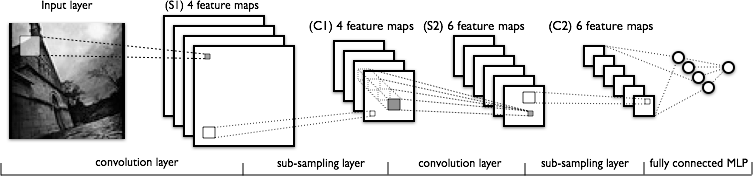
\includegraphics[scale=0.5]{convnet.png}
\end{figure}

\end{frame}

\begin{frame}{\bf 2D convolution}

\begin{figure}
\centering
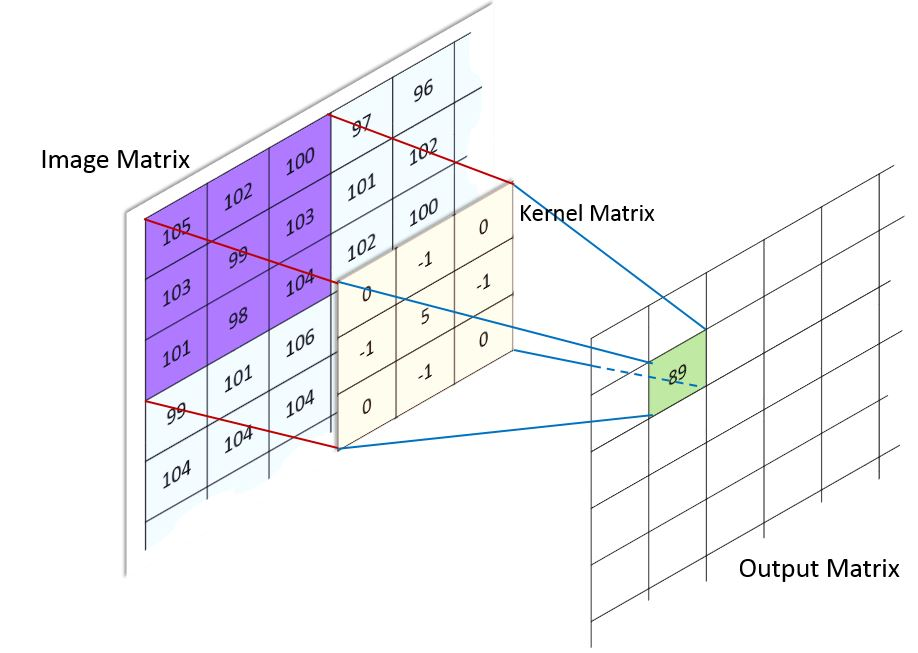
\includegraphics[scale=0.3]{conv_01.jpg}
\end{figure}

\end{frame}

\begin{frame}{\bf 2D convolution}

\begin{figure}
\centering
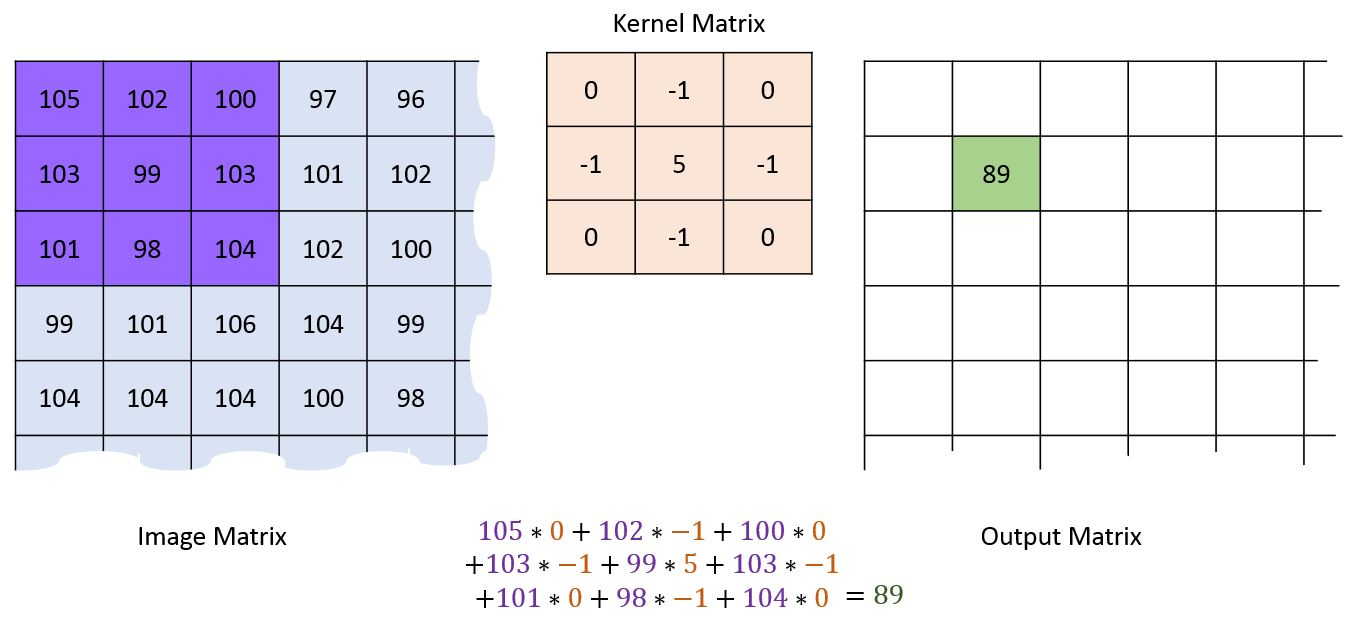
\includegraphics[scale=0.2]{conv_02.jpg}
\end{figure}

\begin{figure}
\centering
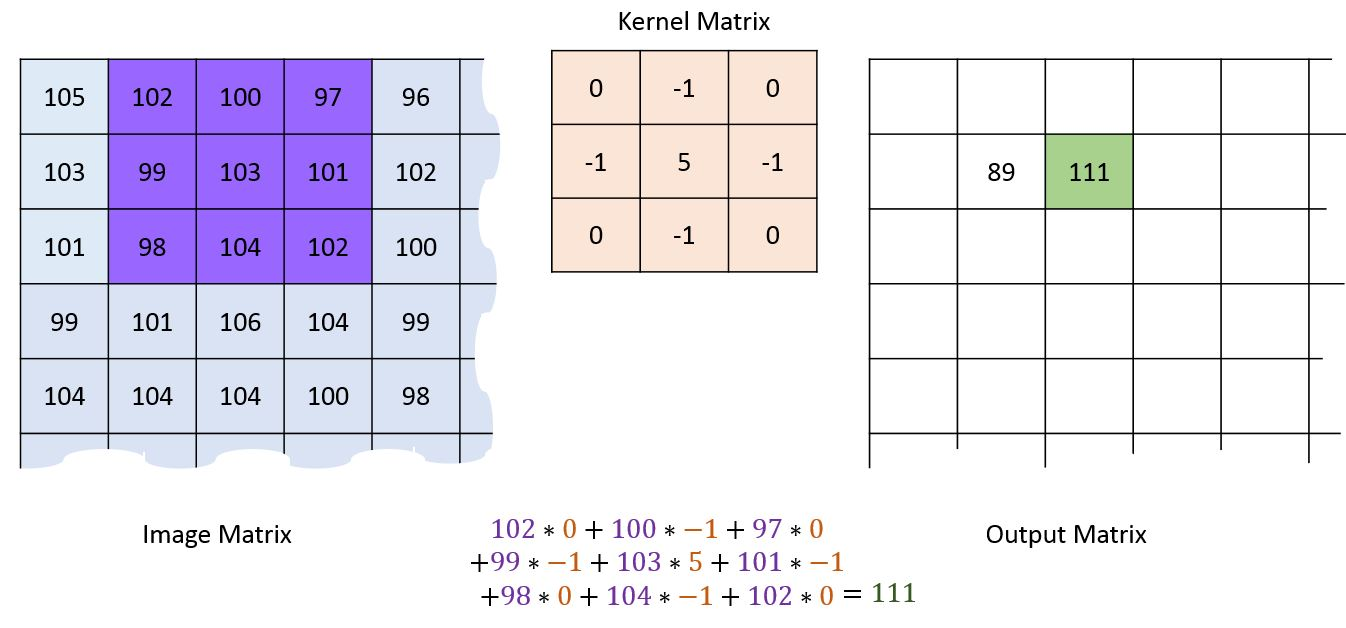
\includegraphics[scale=0.2]{conv_03.jpg}
\end{figure}

\end{frame}




\begin{frame}[fragile]
{\bf 2D convolution}

\lstset{language=C++,
                basicstyle=\tiny,
                emph={int,char,double,float,unsigned},
                emphstyle={\color{blue}},
                numberstyle=\color{green}\tiny,
                keywordstyle=\color{red}\bf\ttfamily,
                stringstyle=\color{red}\ttfamily,
                commentstyle=\color{green}
}

\begin{lstlisting}

for (unsigned y = 0; y <= input_height; y++)
for (unsigned x = 0; x <= input_width; x++)
{
    float sum = 0.0;

    for (unsigned ky = 0; ky < kernel_height; ky++)
    for (unsigned kx = 0; kx < kernel_width; kx++)
    {
      sum+= w[ky][kx]*input[y + ky][x + kx];
    }

    output[y][x] = sum;
  }

\end{lstlisting}
\end{frame}



\begin{frame}[fragile]
{\bf 2D convolution - multiple filters and channels}

\lstset{language=C++,
                basicstyle=\tiny,
                emph={int,char,double,float,unsigned},
                emphstyle={\color{blue}},
                numberstyle=\color{green}\tiny,
                keywordstyle=\color{red}\bf\ttfamily,
                stringstyle=\color{red}\ttfamily,
                commentstyle=\color{green}
}

\begin{lstlisting}

for (unsigned filter = 0; filter < filters_count; filter++)
for (unsigned y = 0; y <= input_height; y++)
for (unsigned x = 0; x <= input_width; x++)
{
    float sum = 0.0;
    for (unsigned ch = 0; ch < channels_count; ch++)
    for (unsigned ky = 0; ky < kernel_height; ky++)
    for (unsigned kx = 0; kx < kernel_width; kx++)
    {
      sum+= w[filter][ch][ky][kx]*input[ch][y + ky][x + kx];
    }

  output[filter][y][x] = sum;
}

\end{lstlisting}
\end{frame}




\begin{frame}[fragile]
{\bf Learning weights}

\lstset{language=C++,
                basicstyle=\tiny,
                emph={int,char,double,float,unsigned},
                emphstyle={\color{blue}},
                numberstyle=\color{green}\tiny,
                keywordstyle=\color{red}\bf\ttfamily,
                stringstyle=\color{red}\ttfamily,
                commentstyle=\color{green}
}

\begin{lstlisting}

for (unsigned filter = 0; filter < filters_count; filter++)
for (unsigned y = 0; y <= input_height; y++)
for (unsigned x = 0; x <= input_width; x++)
{
    float err = error[filter][y][x];

    for (unsigned ch = 0; ch < channels_count; ch++)
    for (unsigned ky = 0; ky < kernel_height; ky++)
    for (unsigned kx = 0; kx < kernel_width; kx++)
    {
        float dif = err*input[ch][y + ky][x + kx];
        w[filter][ch][ky][kx]+= dif*learning_rate;
    }
}


\end{lstlisting}
\end{frame}


\begin{frame}{\bf Pooling}

\begin{figure}
\centering
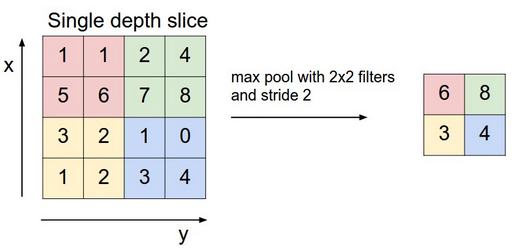
\includegraphics[scale=0.5]{maxpool.png}
\end{figure}

\end{frame}

\begin{frame}{\bf GoogleNet - inception}

\begin{figure}
\centering
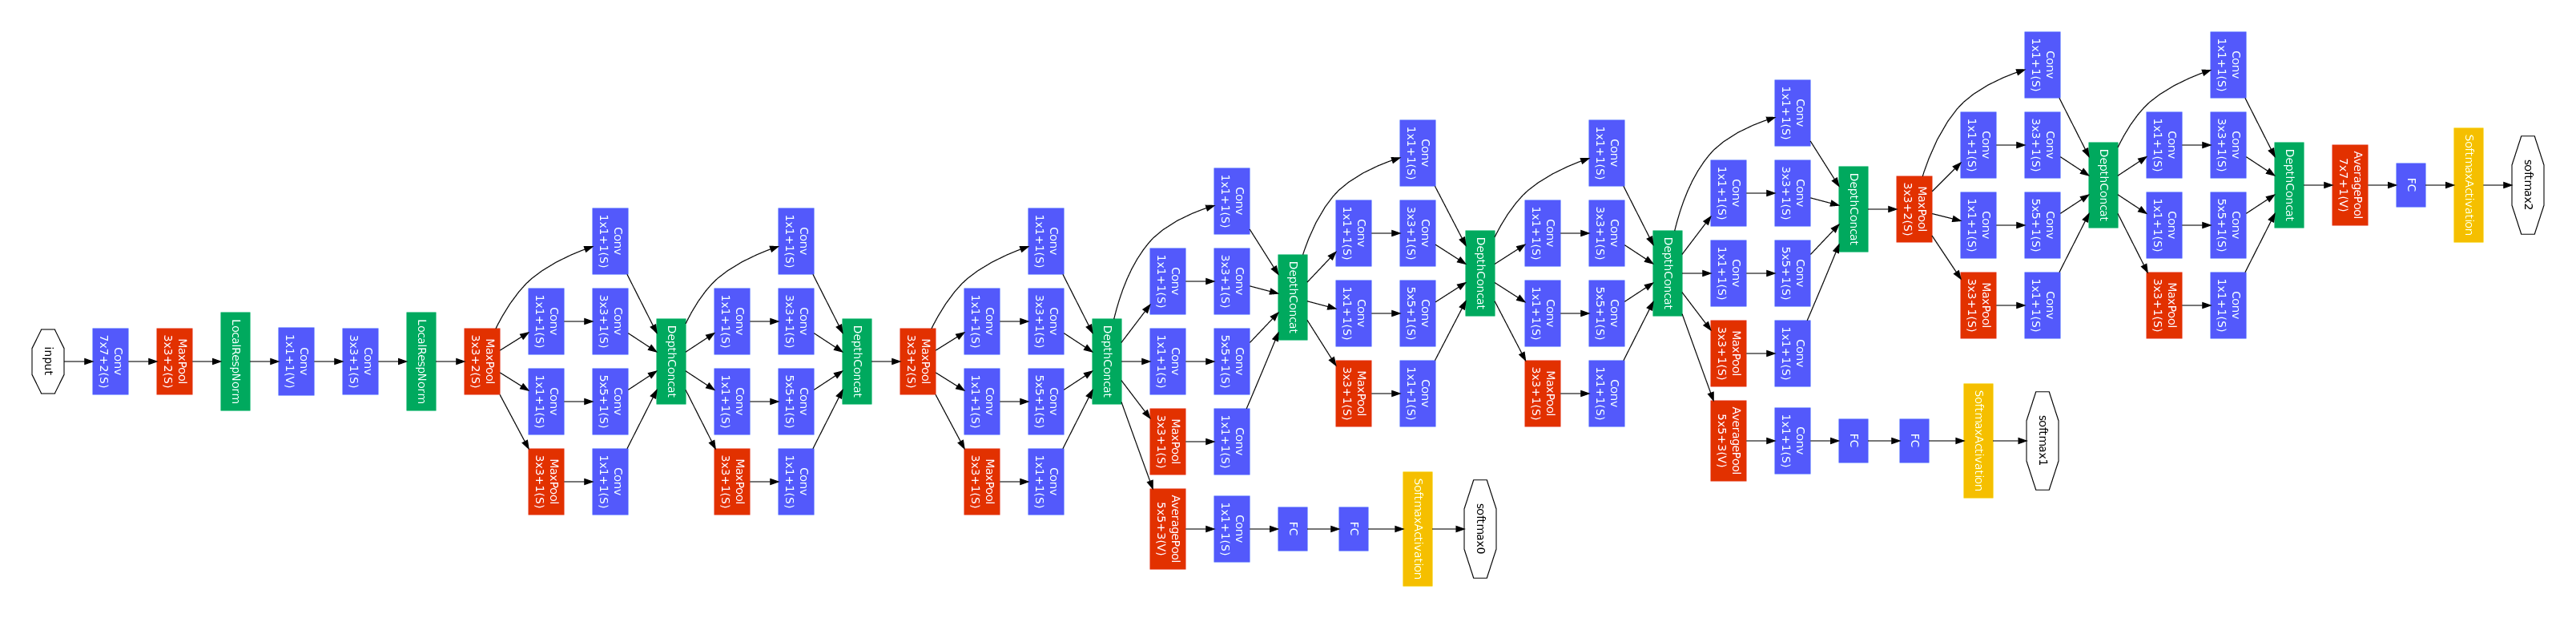
\includegraphics[scale=0.1]{googlenet.png}
\end{figure}

\end{frame}


\begin{frame}{\bf Resnet}

\begin{figure}
\centering
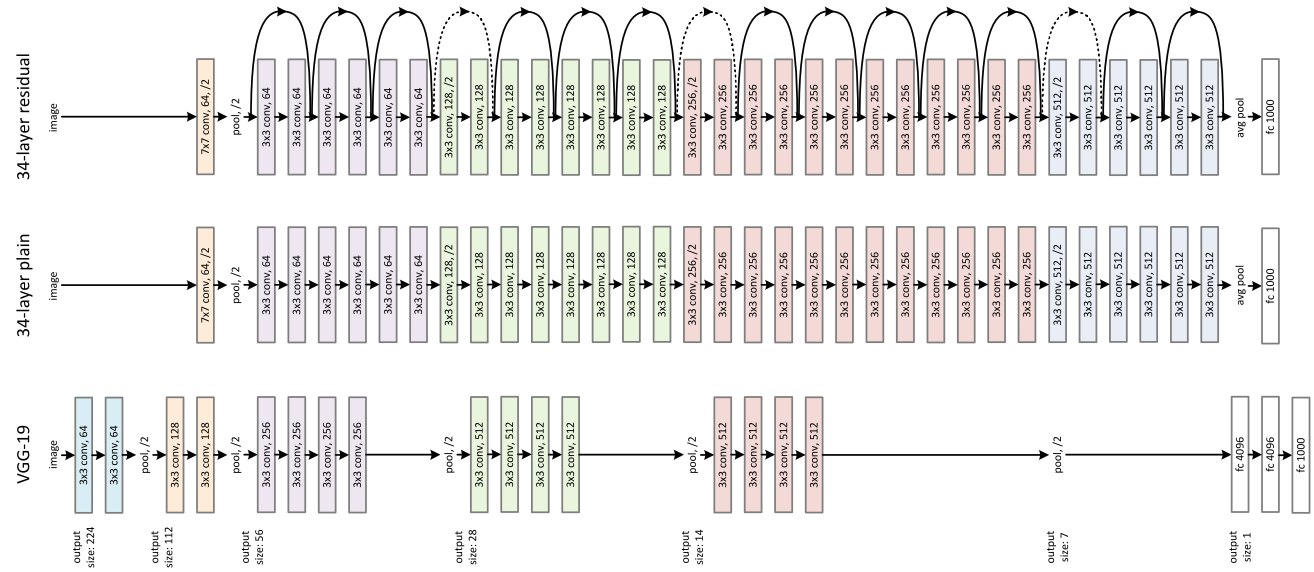
\includegraphics[scale=0.2]{resnet.png}
\end{figure}

\end{frame}



%-------------------------------------------------------------------------------------
\begin{frame}{\bf Q\&A}

\begin{figure}[ht]
\begin{center}
\begin{minipage}{0.8\linewidth}
\begin{center}
 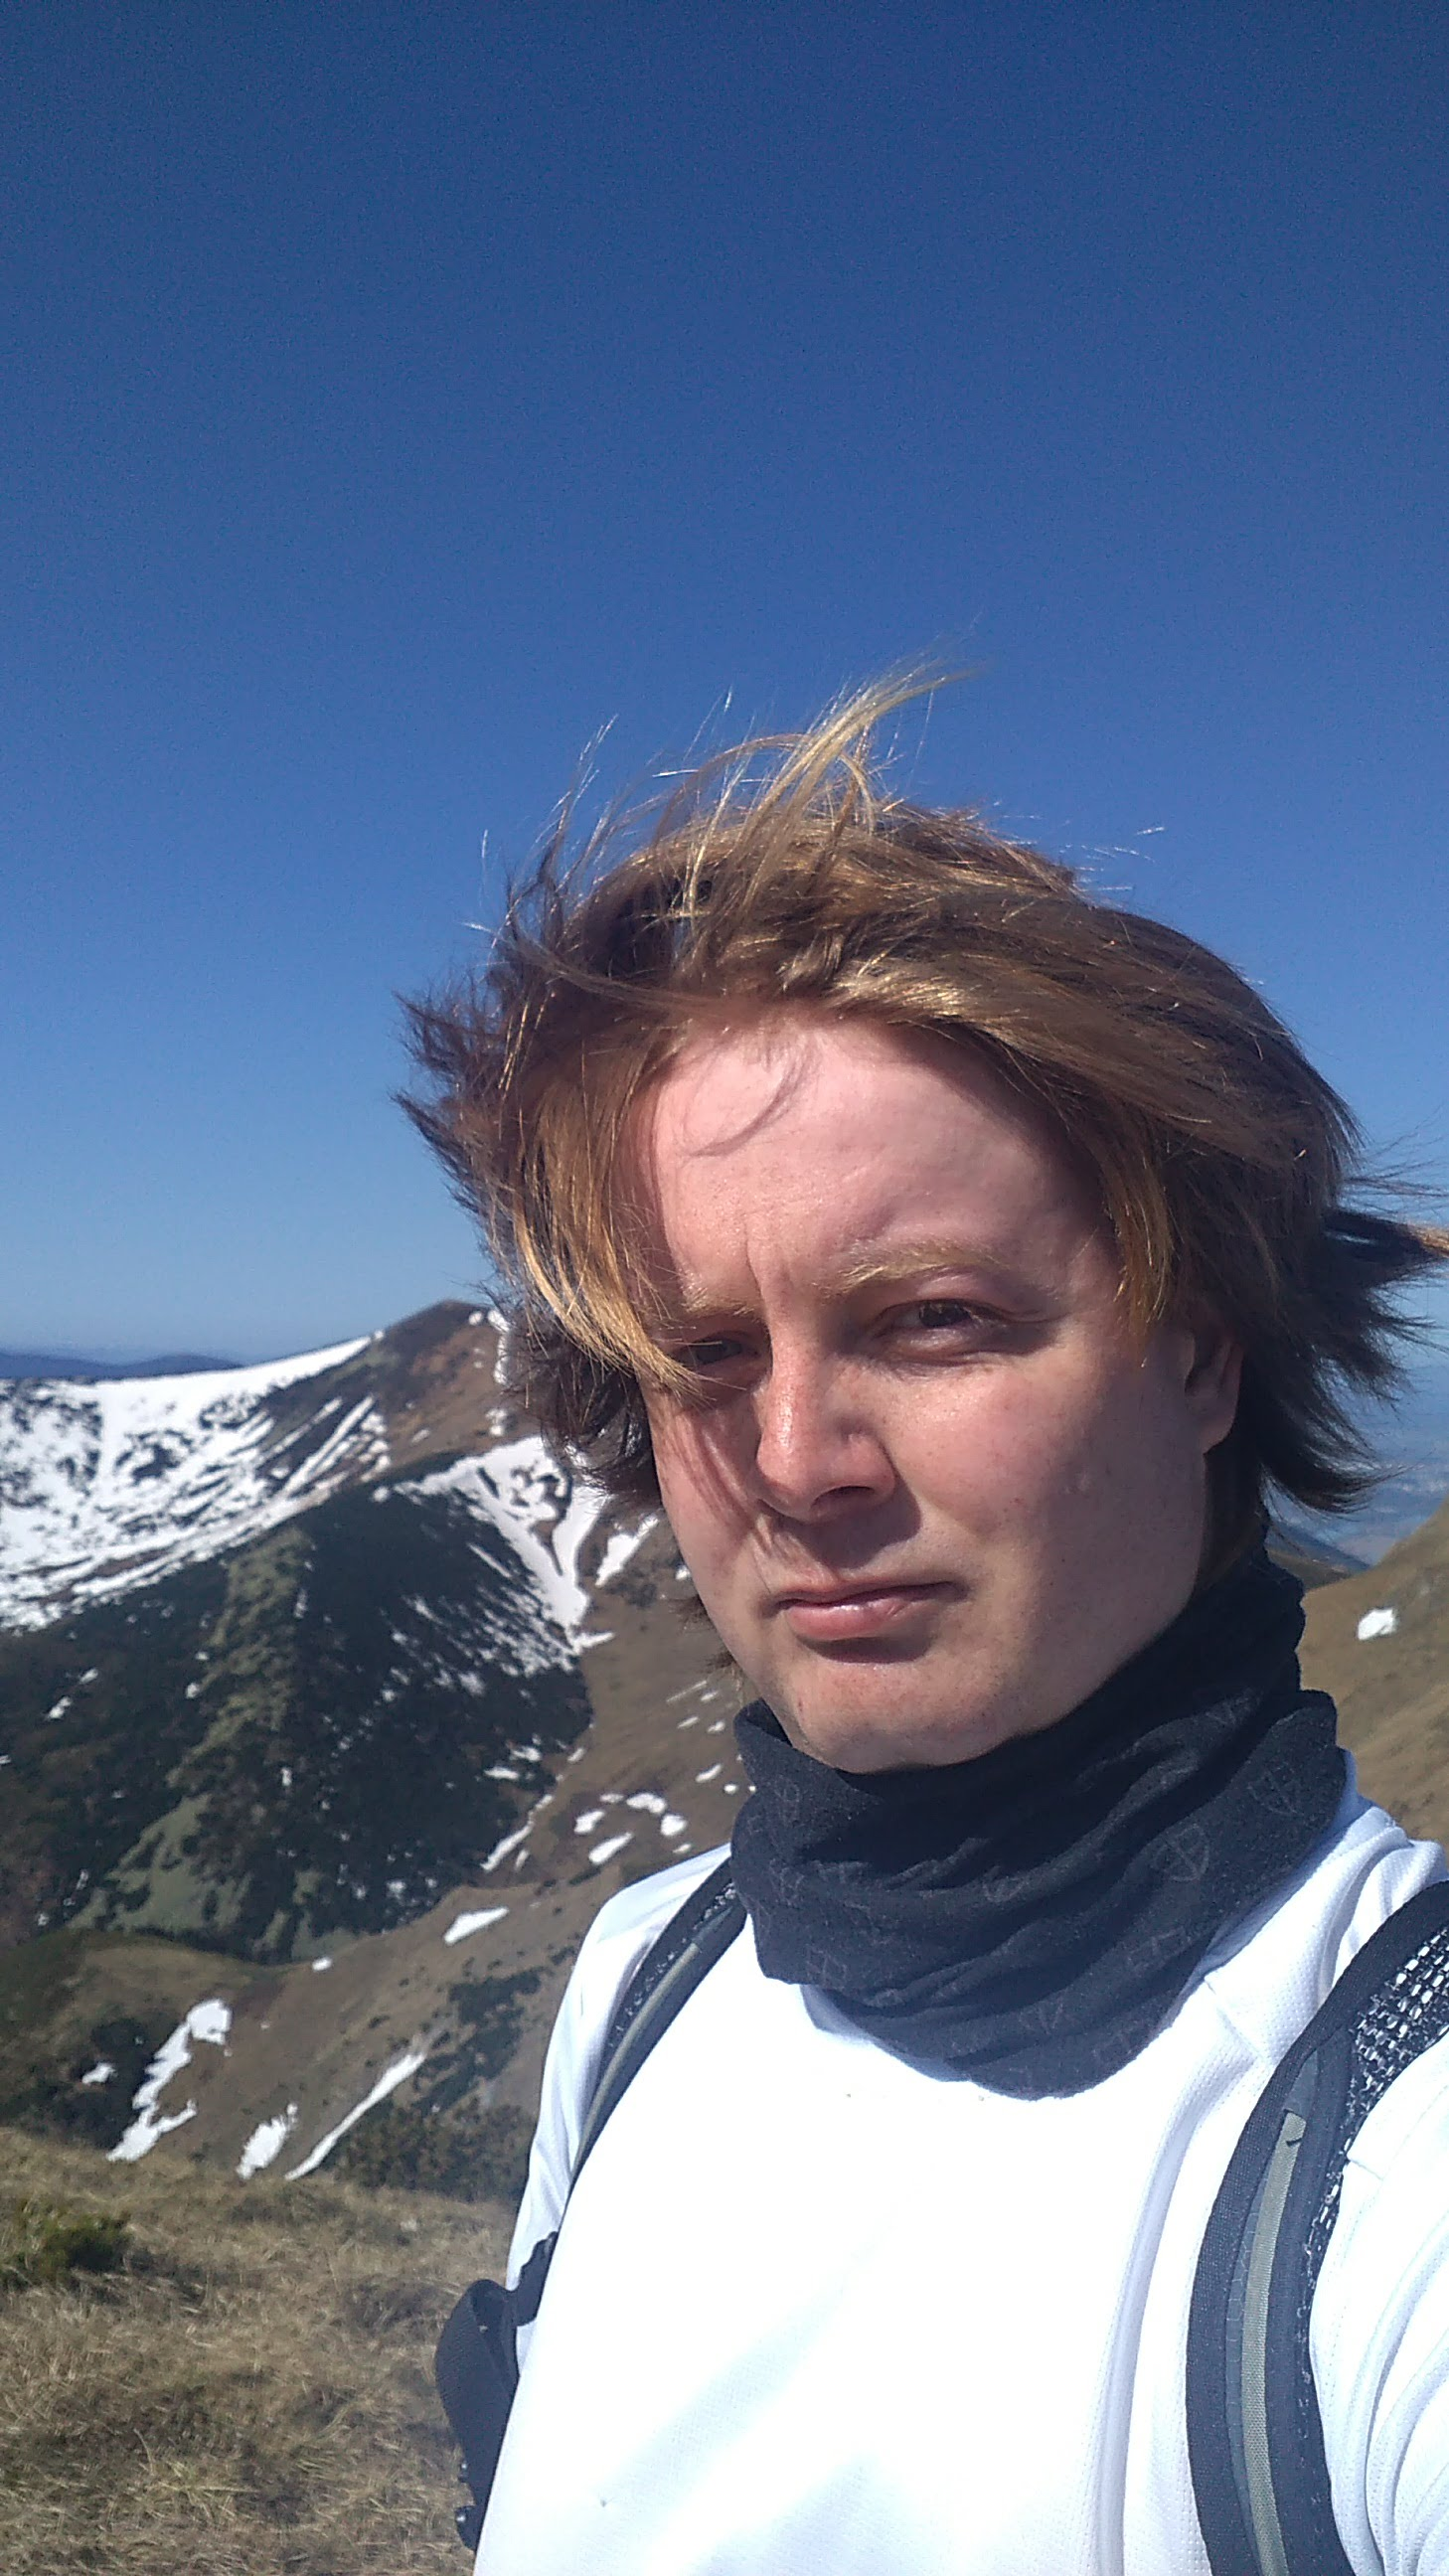
\includegraphics[width=0.35\textwidth]{../../pictures/me3.jpg}
\end{center}
\end{minipage}
\end{center}
\end{figure}

\url{https://github.com/michalnand/robotics}
\url{https://github.com/michalnand/machine\_learning}

\centerline{michal.nand@gmail.com}

\end{frame}

\end{document}
